\chapter{Fundamentos do Layout de Página}
À primeira vista, uma única página de um livro ou outro material impresso consiste em margens, um cabeçalho, um corpo de texto e um rodapé. Mais precisamente, há também um espaço entre a área do cabeçalho e o corpo do texto, bem como entre o corpo e o rodapé. O corpo do texto é chamado, no jargão de tipógrafos e compositores, de área de tipo. A divisão dessas áreas, bem como suas relações entre si e com o papel, é chamada de layout de página.

Vários algoritmos e métodos heurísticos para construir uma área de tipo apropriada foram discutidos na literatura. Essas regras são conhecidas como os “cânones da construção de páginas”. Uma abordagem frequentemente mencionada envolve diagonais e suas interseções. O resultado é que a proporção da área de tipo corresponde às proporções da página. Em um documento de um lado, as margens esquerda e direita devem ter larguras iguais, enquanto a proporção das margens superior e inferior deve ser 1:2. Em um documento frente e verso (por exemplo, um livro), no entanto, toda a margem interna (a margem na lombada) deve ter o mesmo tamanho que cada uma das duas margens externas; em outras palavras, uma única página contribui com apenas metade da margem interna.

No parágrafo anterior, mencionamos e enfatizamos a página. Muitas vezes, pensa-se erroneamente que o formato da página é o mesmo que o formato do papel. No entanto, se você olhar para um documento encadernado, poderá ver que parte do papel desaparece na encadernação e não faz mais parte da página visível. Para a área do tipo, no entanto, não é o formato do papel que é importante; é a impressão da página visível para o leitor. Assim, fica claro que o cálculo da área do tipo deve levar em conta o papel “perdido” na encadernação e adicionar essa quantidade à largura da margem interna. Isso é chamado de correção de encadernação. A correção de encadernação é, portanto, calculada como parte da medianiz, mas não da margem interna visível.

A correção de encadernação depende do processo de produção e não pode ser definida em termos gerais. Portanto, é um parâmetro que deve ser redefinido para cada projeto. Na impressão profissional, esse valor desempenha apenas um papel menor, pois a impressão é feita em folhas maiores de papel e depois cortada no tamanho certo. O corte é feito para que as relações acima para a página visível, frente e verso sejam mantidas.

\section*{Layout de dois lados com a construção de caixa da divisão clássica de nove partes, após subtrair uma correção de encadernação:
}
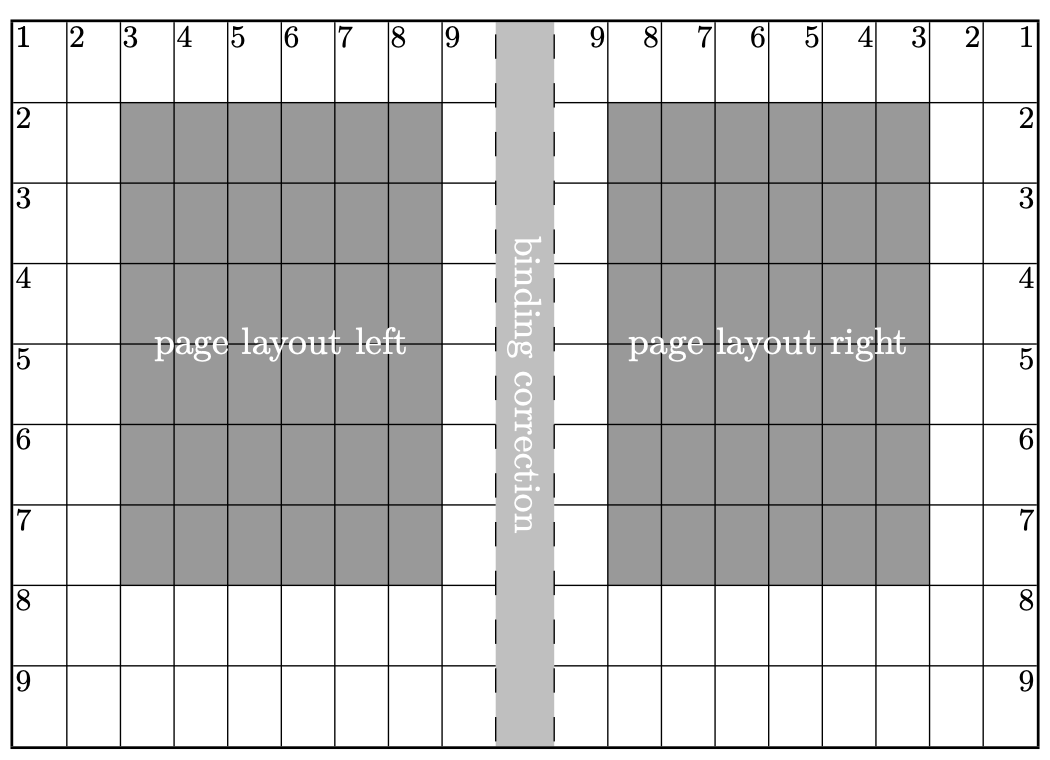
\includegraphics[scale=0.8]{imagem02.png}

O que resta na página é a área de texto. A largura e a altura da área de texto e margens resultam automaticamente do número de linhas e colunas, DIV. Como as margens sempre precisam de três listras, DIV deve ser maior que três. Para que a área de texto ocupe pelo menos o dobro de espaço das margens, DIV deve ser pelo menos nove. Com esse valor, o design também é conhecido como a divisão clássica de nove partes.

No \KOMAScript\ esse tipo de design é implementado com o pacote typearea, onde a margem inferior pode remover quaisquer frações de uma linha para cumprir com a restrição para a altura da área de tipo mencionada no parágrafo anterior e, assim, reduzir o problema mencionado com \verb|\flushbottom|. Para papel A4, DIV é predefinido de acordo com o tamanho da fonte (veja tabela 2.2, página 36). Se não houver correção de encadernação (BCOR = 0 pt), os resultados correspondem aproximadamente aos valores da tabela 2.1, página 35.

Além dos valores predefinidos, você pode especificar BCOR e DIV como opções ao carregar o pacote (veja a seção 2.4, começando na página 33). Há também um comando para calcular a área do tipo explicitamente fornecendo esses valores como parâmetros (veja também a seção 2.4, página 39).

\begin{verbatim}
            \typearea[BCOR]{DIV}
            \recalctypearea
\end{verbatim}


O pacote typearea pode determinar automaticamente o valor ideal de DIV para a fonte e entrelinhamento usados.

\section{Dimensões da área de tipo dependentes de DIV para A4 independentemente de \texttt{\char`\\topskip} ou BCOR}


\begin{figure}[ht]
    \centering
    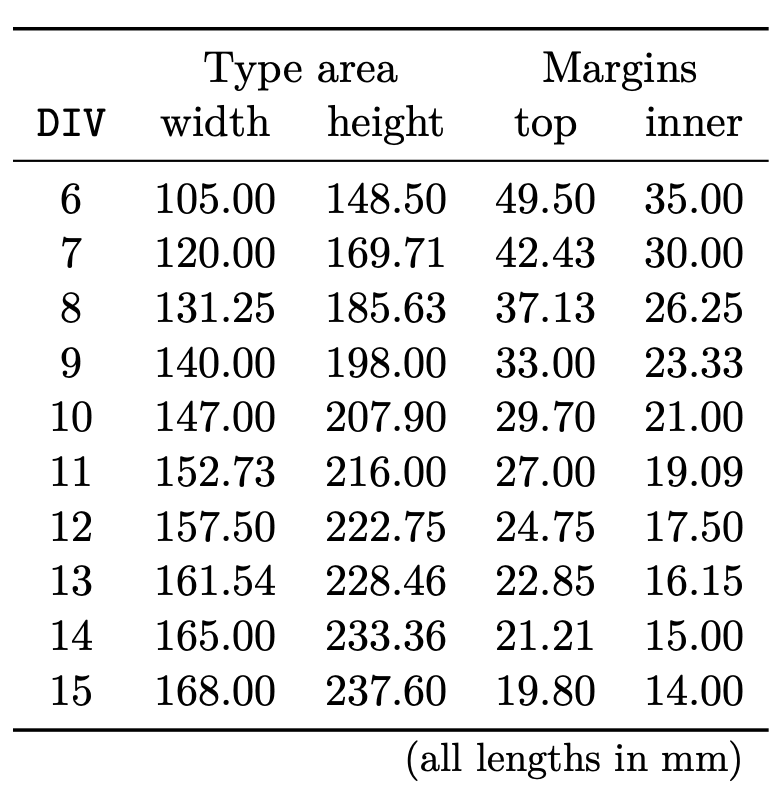
\includegraphics[width=0.45\linewidth]{tab2_1.png}
    \caption{Tabela 2.1 do Manual}
    \label{fig:tab2_1l}
\end{figure}

\section{DIV defaults for A4 in all \KOMAScript\ classes:}
\begin{figure}[hb]
    \centering
    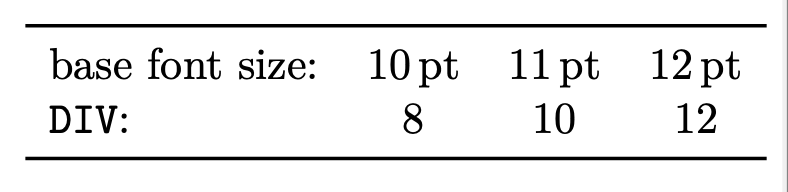
\includegraphics[width=0.5\linewidth]{tab2_2.png}
    \caption{Tabela 2.2 do Manual}
    \label{fig:tab2_2}
\end{figure}

